\documentclass[a4paper, 12pt]{article}
\usepackage{ctex}
\usepackage{graphicx}
\usepackage{subfigure}
\usepackage{booktabs} %三线表
\usepackage[unicode,
colorlinks,
linkcolor=blue,
anchorcolor=red,
citecolor=green
]{hyperref}
\usepackage{xcolor}
\usepackage[super,square]{natbib}
\usepackage{indentfirst}
\usepackage{amsmath}
\usepackage[ruled,vlined]{algorithm2e}
\usepackage{caption}
\captionsetup{hypcap=true, font={small}} %正确跳转到图片

%%%% 下面的命令重定义页面边距,使其符合中文刊物习惯 %%%%
\addtolength{\topmargin}{-54pt}
\setlength{\oddsidemargin}{0.63cm}  % 3.17cm - 1 inch
\setlength{\evensidemargin}{\oddsidemargin}
\setlength{\textwidth}{14.66cm}
\setlength{\textheight}{24.00cm}    % 24.62

%%%% 下面的命令设置行间距与段落间距 %%%%
\linespread{1.4}
% \setlength{\parskip}{1ex}
\setlength{\parskip}{0.5\baselineskip}

\begin{document}
\bibliographystyle{unsrt,plain}%abbrv,plain,alpha
%%%% 定理类环境的定义 %%%%
\newtheorem{example}{例}             % 整体编号
\newtheorem{theorem}{定理}[section]  % 按 section 编号
\newtheorem{definition}{定义}
%\newtheorem{algorithm}{算法}
\newtheorem{axiom}{公理}
\newtheorem{property}{性质}
\newtheorem{proposition}{命题}
\newtheorem{lemma}{引理}
\newtheorem{corollary}{推论}
\newtheorem{remark}{注解}
\newtheorem{condition}{条件}
\newtheorem{conclusion}{结论}
\newtheorem{assumption}{假设}

%%%% 重定义 %%%%
\renewcommand{\contentsname}{目录}  % 将Contents改为目录
\renewcommand{\abstractname}{摘要}  % 将Abstract改为摘要
\renewcommand{\refname}{参考文献}   % 将References改为参考文献
\renewcommand{\indexname}{索引}
\renewcommand{\figurename}{图}
\renewcommand{\tablename}{表}
\renewcommand{\appendixname}{附录}
\renewcommand{\algorithmcfname}{算法} %针对 algorithm2e 宏包

%%%% 定义标题格式,包括title,author,affiliation,email等 %%%%
\title{基于多模态融合的手势分割与识别}
\author{张芮溟\\
 同济大学控制科学与工程系,上海,201804;\\[2ex]}
\date{2016年12月}

\maketitle

\begin{abstract}
  本文首先介绍了一种叫做深度动态神经网络的手势分割与识别方法,该方法能够同时有效利用两种无法直接进行融合的观测信息——骨骼数据和图像RGBD数据。在对骨骼数据的利用上,该方法使用了高斯伯努利深度置信网络(DBN)获取骨骼动态信息,在对图像信息的提取上,该方法利用了3D-CNN网络获取高维的特征描述,随后该方法将两个网络的有效参数作为预训练参数整合进一个大的融合网络,进一步调整网络权值。以上过程即是对观测概率的建模过程,我们对观测概率套用隐马尔科夫模型就可以得到一个可能性最高的手势序列。通过对实验结果的分析,针对该方法存在的缺陷,本文对模型中的CNN网络做了一定的改进,提高了预测准确度。
  \\
  \\
  \textbf{关键字:} 手势分割与识别~~深度学习~~DBN~~3D-CNN~~HMM
\end{abstract}

\section{引言}
本文关注的是视频中人类手势的识别问题。人类的行为识别在近些年来逐渐引起了人们的广泛关注,因为其在很多环境中都有一定的潜在应用价值,它可以被用于监视视频中人类的异常行为如打架、盗窃、老人摔倒等等,在安防领域具有很大的发展前景,除此之外,它还可以用于用户接口的设计,如手势控制智能家电的开关等等。
本文的方法主要是针对连续不重复视频动作序列中人类手势进行标记,这里的非重复动作主要是相对于行走、跑步这样循环往复的动作来说。

传统的人类行为识别方法大多基于两个步骤:首先在原始的输入信息中提取计算复杂的人工特征,然后基于我们获取到的人工特征选择一个分类器进行学习。
但是在现实情况中,我们很难主观地判断哪些特征是比较重要的,因为特征的选择和具体的问题高度依赖。

基于以上缺点我们提出用神经网络来解决这个问题,受到语音识别方法的启发\cite{p1},通过在隐马尔科夫架构中整合进一个深度神经网络,如图\ref{fig:1}所示,我我们可以同时实现一段视频序列中人类手势的有效分割与识别。具体来说,本方法主要包括一下几个部分:
\begin{itemize}
\item 设计了一个深度置信网络来提取骨骼数据的高级动态特征,并用其来推算一个观测概率。
\item 提出通过3D卷积操作来提取视频数据的时间和空间特征。
\item 提出两种多模态融合策略将两种模态的数据有机地结合起来,提高信息利用率以及预测准确性。
\end{itemize}
\begin{figure}[ht]
  \centering
  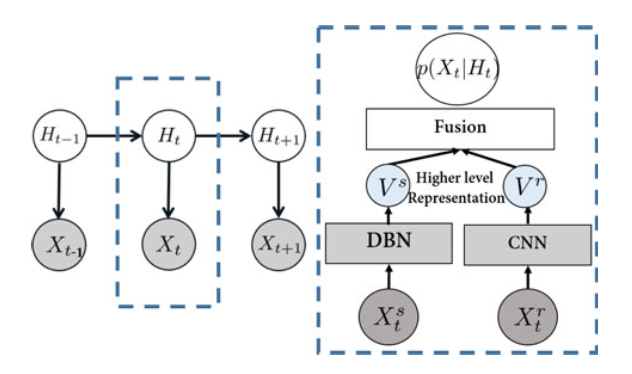
\includegraphics[width=8cm]{HMM.png}
\caption{左图是对隐马尔科夫模型的时域建模,其中输出概率$p(X_t|H_t)$由右侧的网络得到}
  \label{fig:1}
\end{figure}

\section{模型构建}
\subsection{隐马尔科夫模型}
\label{ss:1}
对于一段由很多复杂帧组成的手势序列,很显然将这么大的数据量作为一个整体直接作为网络的输入是不现实的,为了尽可能减少可训练参数,我们只能给网络输入有限帧,这就意味着我们只能通过网络提取到比较低级的动作特征。这些特征很难指导我们直接通过分类器获得正确的手势类别。因此为了提高预测准确性,我们不直接将分类器接在网络的最后用来输出手势类别,而是引入隐马尔科夫模型来描述高级的动作特征,进而得到发生概率最大的手势类别作为我们的预测结果。

隐马尔可夫模型(HMM)是一种统计模型,它用来描述一个含有隐含未知参数的马尔科夫过程。一个隐马尔科夫模型的状态不能直接观察到,而是要通过观测向量序列观察得到,每个观测向量都符合某种概率密度分布。在我们的模型中,用$X_t$表示可观测序列,它包含骨骼数据$X^s_t$和RGB-D数据$X^r_t$,用$H_t$表示隐藏序列,它表示手势中的一个状态。一个复杂的手势通常由几个阶段构成,本文中统一将手势分成五个阶段,每个阶段称为一个状态。除此之外我们还设置一个过渡状态用来表示手势与手势间的过渡阶段。图\ref{fig:2}展示了手势内部各状态及手势间状态的转换关系。由于实验采用的数据集包含20种手势,因此隐藏状态$H_t$共有101个。那么在隐马模型下,观测状态和隐藏状态的联合概率分布可以用如下公式来表示:
\begin{equation}
  p(H_{1:T}, X_{1:T})= p(H_1)p(X_1|H_1)\prod_{t=2}^{T}{p(X_t|H_t)p(H_t|H_{t-1})}
\end{equation}
$p(H_1)$是初始概率,$p(H_t|H_{t-1})$是隐藏状态间的状态转移概率, $p(X_t|H_t)$ 是输出概率,它表示隐含状态到可见状态的概率分布,由于隐含状态包含了高级的动态特征,因此它与可观测状态之间的关系不能简单通过统计方法获得,而是要通过我们设计的网络学习获得,见图\ref{fig:2}。前面两种概率则可以基于先验知识以及对数据的统计结果得到。
\begin{figure}[ht]
  \centering
  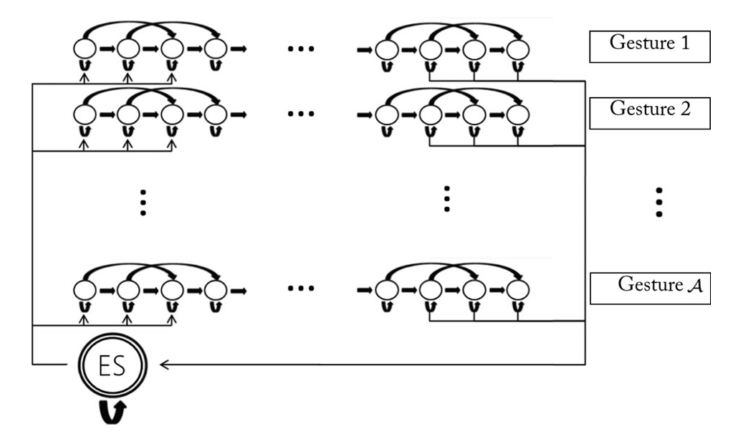
\includegraphics[width=8cm]{stateDiagram.png}
  \caption{隐藏状态转换关系}
  \label{fig:2}
\end{figure}

已知了观测序列$X_t$ ,隐藏状态集合 $N_H$,初始概率 $\pi_i$,状态转移概率 $a_{H_i,H_j}$,以及输出概率 $p(X_t|H_t)$,想要推算隐藏状态序列,这就是隐马模型最经典的问题之一——解码问题,本文选用最常用的维特比算法来进行隐藏状态解码。

该算法的思想就是通过动态规划,寻找每一步的局部最优解,从而实现最短路径。
用递推方程来描述该算法如下:
\begin{equation}
  \delta_{1,h} = p(X_1|H_k)*\pi_k
\end{equation}
\begin{equation}
  \delta_{t,h}=p(X_t|H_k)*max_{y\in N_H}(a_{H_{k-1},H_k}*\delta_{t-1,h})
\end{equation}

通过前$t$个观测结果得到的每个隐藏状态 $H_k$的概率分布为 $\delta_{t,h}$,当前的 $N_H$ 个概率分布中占有最大概率分布的隐藏状态就作为这一步的最优状态,最终我们可以得到一系列的最优状态,这就是我们所要求的隐藏序列。

\subsection{DBN用于骨骼模块}
\subsubsection{骨骼数据的预处理}
原始的骨骼数据只包含某一时刻关节的静态姿态信息,为了使得训练网络的学习更有效,本文对骨骼数据首先进行了预处理,提取到关节的初步动态特性(位置、速度及加速度信息),根据文献\cite{p2},这个操作也可以在网络内部进行——在网络的第一层首先设置一个固定权值参数的硬连接层,相当于基于先验知识对训练网络进行了引导。本文认为前者的数据预处理速度更快。

原始数据集包含全身21个关节的数据信息,由于手势只引入了上半身的动作,我们仅处理上半身的十一个关节的数据,那么在时间节点$t$,原始的骨骼数据输入可以表示为$x_t^s=[x_t^{s,1},...,x_t^{s,N_j}]$,其中, $N_j=11$ 。
每一个关节的数据 $x_i$又是一个一维的向量,包含了世界坐标、旋转角度和像素坐标等信息。

\begin{equation}
  f_t^{cc}=x_t^{s,i}-x_t^{s,j}|i,j = 1,2,...,N_j;i\neq j
\end{equation}
\begin{equation}
  f_t^{cp}=x_{t+1}^{s,i}-x_t^{s,i}|i = 1,2,...,N_j
\end{equation}
\begin{equation}
  f_t^{ca}=x_{t+1}^{s,i}-2*x_t^{s,i}+x_{t-1}^{s,i}|i = 1,2,...,N_j
\end{equation}

按照以上公式进行骨骼动态特性的提取,可以得到特征向量$f_t=[f_t^{cc}, f_t^{cp}, f_t^{ca}]$,该向量共含有$N_f = N_j \times (\frac{N_j}{2}+N_j +N_j)*3=891$个元素,那么骨骼网络的输入节点数也就是891个。

\subsubsection{深度置信网络}
用来处理骨骼数据的DBN网络实际上是由多层的RBM堆叠以及一个softmax输出层构成的,一个普通的RBM网络如图\ref{fig:rbn}所示,共有2层,第一层称为可视层,是输入层,第二层是隐含层,也就是特征提取层。之所以利用RBM网络能够提取数据的特征,是因为当输入 $v_m$ 的时候,通过 $p(h|v)$ 可以得到隐藏层 $h_n$,而得到隐藏层 $h_n$ 之后,通过 $p(v|h)$ 又能够得到可视层 $v_m'$,通过调整参数,我们能够使得从隐藏层得到的可视层与原来的可视层一样,那么此时得到的隐藏层就是可视层另外一种表达,也就是说隐含层提取到了可视层的特征。
\begin{figure}[ht]
  \centering
  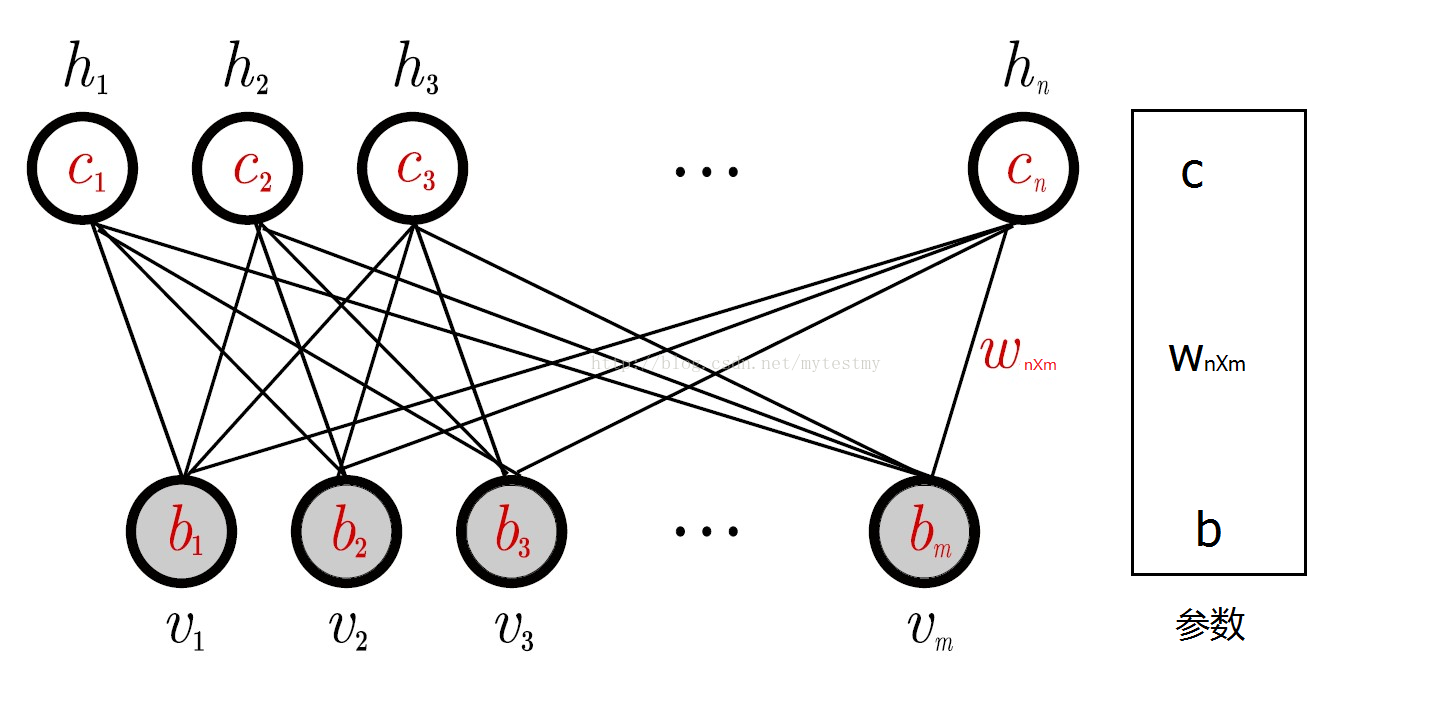
\includegraphics[width=8cm]{RBM.png}
  \caption{\label{fig:rbn}DBN网络架构}
\end{figure}

网络的参数值通过最小化损失函数值的方法来求解,与传统的RBM有点不同的是,可视层节点的输出不再是离散的或是二值化的值,而是具有连续值的骨骼数据,因此第一层RBM的能量函数求解公式较标准的公式有些改动:

\begin{equation}
  E(f,h;\theta) = -\sum_i{\frac{(f_i-b_i)^2}{2\sigma_i^2}} - \sum_i{}\sum_j{W_{ij}h_j\frac{f_i}{\sigma_i}} - \sum_{j=1}{a_jh_j}
\end{equation}

其中$\theta=\{W,b,a\}$,是网络的参数,分别表示可视层与隐藏层之间的权值矩阵和偏移量。前向和后向的条件概率分布分别用逻辑函数和正态分布来建模:
\begin{equation}
  P(h_j=1|f) = g(\sum_i{W_{ij}f_i+a_j})
\end{equation}
\begin{equation}
  P(f_j=f|h) = N(f|\mu_i,\sigma^2_i)
\end{equation}


本文对骨骼数据的处理分为两步,首先通过无监督学习的方法逐层的训练RBM网络参数,然后用这些参数来初始化DBN网络,通过监督学习的方式对参数进行调整。实验中选用每层的节点数为 $[N_f,2000,2000,1000,N_H]$。

\subsection{3D-CNN用于RGB-D模块}
\subsubsection{RGB-D数据的预处理}
与对骨骼数据进行预处理的思路一样,手是我们最关心的部位,而两只手中位置相对较高的手往往是做出动作的一个,并且当两只手共同完成一个手势时,通常会做镜像的动作。基于以上共识,本文首先将高像素图像做了剪切和压缩,分别分割成了只包含上半身和只包含一只手的具有40*40个像素点的图片,接着基于人的位置对图片做了镜像处理,这样图片的任意一半就包含了所有的动作信息。

\subsubsection{3D-CNN网络}
CNN网络用在图片处理中具有十分突出的优点,它可以直接作用于无标记数据,经过交替设计的滤波器和局部池化层提取的复杂的高级特征,但是传统的2D-CNN作用于单帧图片,不能有效学习到连续帧间的运动信息\cite{p7}。因此为了有效提取运动特性,本文提出了3D-CNN的方法,同时在空间和时间维度上对一组图片做特征提取。其与CNN最大的差异在于输入数据不再是单幅图像,而是多幅图像堆叠成的立方块,相应地特征提取层的卷积核也应变成三维,其余的特性与CNN完全一致。特征图的计算公式如下式所示:
\begin{equation}
  v_{i,j}^{x,y} = max(0, (b_{ij} + \sum_m \sum_{p=0}^{P_i-1} \sum_{q=0}^{Q_i-1} w_{ijm}^{pq}v_{(i-1)m}^{(x+p)(y+q)}))
\end{equation}

本文的3D-CNN网络架构如图\ref{fig:3}所示,网络的输入共有4个通道:手和上半身分别对应的深度图和灰度图,在第一次卷积操作后将灰度图和深度图合并为一个通道。经过3层卷积和3层最大值池化将特征维度降为5×5×1的低维特征图,然后将全部的特征图展开并连在一起,与一个含有1024个节点的全连接层相连接,输出层含有101个节点,与隐马尔科夫的101个隐藏状态相对应。
\begin{figure}[ht]
  \centering
  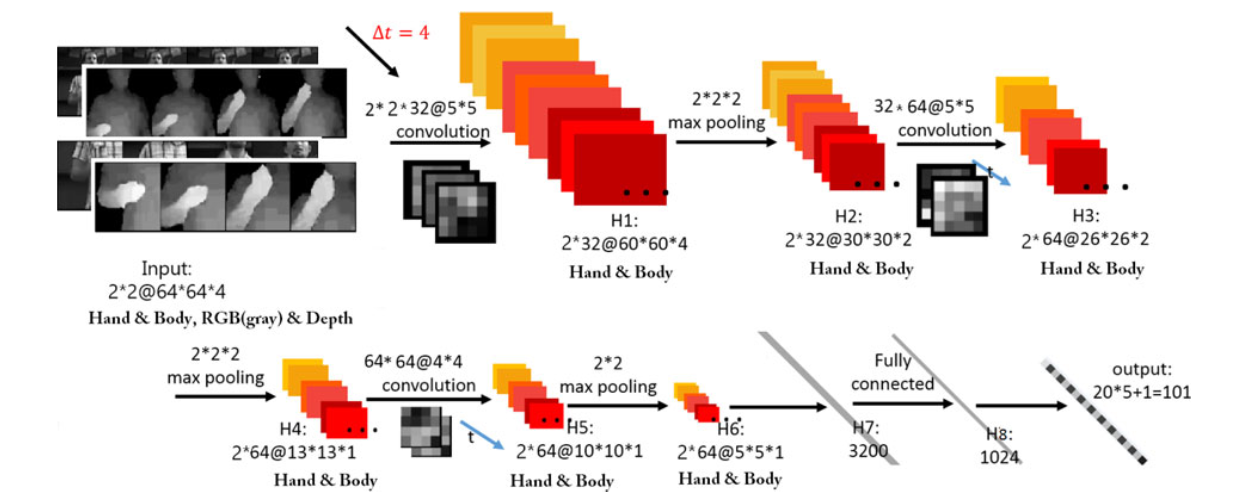
\includegraphics[width=10cm]{cnnArchitecture.png}
  \caption{\label{fig:3}3D-CNN网络架构}
\end{figure}

\subsection{多模态融合}
使用上述任意一种模态的数据都可以独立进行动作特征的提取,并估算出隐马模型所需要的输出概率,但是很显然这会造成大量信息的浪费。因此,为了提高数据的利用率,同时也为了提高预测的准确性,本文将两个网络的输出结果进行融合,得到一个联合的输出概率估计,用于最终序列的解码。

\begin{figure}[ht]
  \centering
  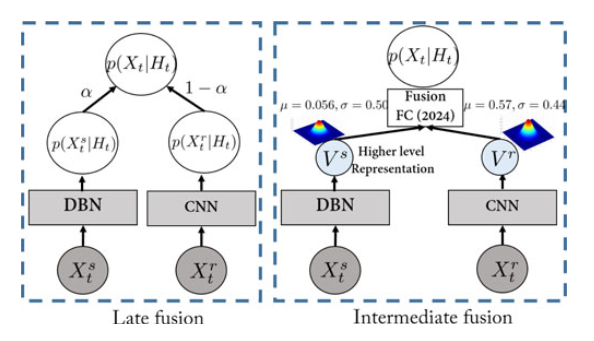
\includegraphics[width=8cm]{fusion.png}
  \caption{\label{fig:4}多模态融合}
\end{figure}

本文给出了两种方法(图\ref{fig:4}),一种是直接对两个网络的输出做线性的叠加,通过调整两个网络输出的权值得到理想的输出概率估计,另一种是对两种模态的高级动作特征进行融合,将两个网络的全链接层连在一起,直接得到交叉了两种模态特征的联合输出概率估计。实验发现前者的预测效果略优于后者,因此本文选用了第一种方法。

\subsection{本文的改进}
可以看到原方法对网络方法的运用还停滞在最初级阶段,不能有效的利用大量的信息。针对原方法的缺点,本文着重对CNN网络进行了改进,提高了RGBD模块的预测准确性,进而提高了整体模型的准确性。具体来说,主要包含如下几点改进:

\begin{itemize}
\item 独立处理灰度和深度信息。在卷积操作的第一层,原方法就将来自两个独立通道的深度信息和灰度信息合并为一个通道,参考文献\cite{p5},每个通道的信息应保留到最后才能最有效的提取到高级特征。
\item
参考文献\cite{p3},本文引入了“模型规则化”这一概念。考虑到控制计算复杂度,我们将CNN网络的输入限定在4个帧。但是通常来说一个手势含有几十帧到几百帧,显然有限的输入维度使得我们很难从中提取到高级的动作信息,因此本文将一系列带有高级行为信息的辅助节点连接在CNN的最后一个隐含层。
\item 可以注意到,经过第一点改进,CNN网络的计算复杂度又进一步提高,为了平衡计算量,同时也为了网络能够学习到更高级的动作特征,本文引入“输入帧步长”这一概念,根据输入手势序列的帧长度动态调整CNN网络输入立方块的帧间隔。
\end{itemize}

\subsubsection{双通道分离卷积}
在原方法的3D-CNN结构中,来自两个独立通道的深度立方块和灰度立方块在做第一层卷积操作时被通过修正线性单元叠加成一幅特征图,这会损失掉一部分特征信息,因此,在改进方法中,我们在两个通道中对灰度立方块和深度立方块分别做卷积操作,在第7个隐含层中将四个通道(还分为手和上半身)的特征向量连接在一起,这样第7层的特征向量维数应该为6400个。

\subsubsection{模型规则化}
考虑到模型参数数量的控制,CNN网络的输入尺寸必然受到限制。我们虽然不能直接通过CNN网络得到高级的动作特征,但是可以通过其他的方法来计算长时间的行为信息,从而实现高级运动特征的提取。然后本文将这个高级的行为特征作为辅助去规则化3D-CNN模型,迫使CNN网络学习到一个非常接近这个高级特征的特征向量。

具体的实现方法如图\ref{fig:5}所示,首先从视频中提取到高级运动特征,接着利用提取到的高级运动特征根据手势类别构造出相应维度的“单词表”,将这一系列的辅助输出节点与CNN的最后一个隐含层相连,然后在训练过程中,使提取的特征更好的逼近这个高层的运动特征向量。

\begin{figure}[ht]
  \centering
  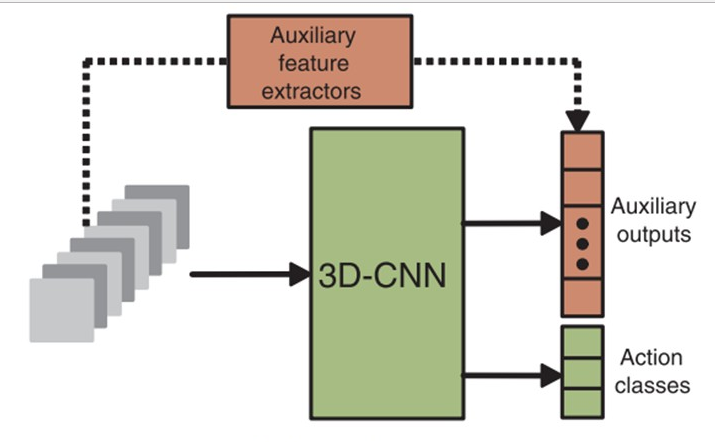
\includegraphics[width=8cm]{regular.png}
  \caption{\label{fig:5}模型规则化}
\end{figure}


高级运动特征的提取,文献\cite{p4}采用了计算稠密SIFT描述子的方法。考虑到对数据集的充分利用,同时避免不必要的计算,本文采用运动图像边缘信息提取高级运动特征。因为数据集中已经给出了每一帧图像的二值化灰度图,实际要做的就是利用canny算子对二值化图像提取边缘。

canny算子是现阶段应用最为广泛而且设计最为理想的边缘检测算法之一\cite{p6},该算法大致的执行流程是:
\begin{enumerate}
\item 求图像与高斯平滑滤波器的卷积:
\begin{equation}
  S[i,j] = G[i,j;\sigma]*I[i,j]
\end{equation}
\item 使用一阶有限查分计算偏导数的两个阵列P与Q:
\begin{equation}
  P[i,j]\approx (S[i,j+1]-S[i,j]+S[i+1,j+1]-S[i+1,j])/2
\end{equation}
\begin{equation}
  Q[i,j]\approx (S[i,j]-S[i+1,j]+S[i,j+1]-S[i+1,j+1])/2
\end{equation}
\item 求出幅值和方位角:
\begin{equation}
  M[i,j] = \sqrt{P[i,j]^2+Q[i,j]^2}
\end{equation}
\begin{equation}
  \theta[i,j] = \arctan(Q[i,j]/P[i,j])
\end{equation}
\item 采用非极大值抑制法细化幅值图像中的屋脊带,只保留幅值局部变化最大的点:
\begin{equation}
  \zeta[i,j] = sector(\theta[i,j])
\end{equation}
\begin{equation}
  N[i,j] = NMS(M[i,j],\zeta[i,j])
\end{equation}
\item 取阈值,将低于阈值的所有值赋0,即可得到图像的边缘阵列。
\end{enumerate}

随机抽取数据集中一帧彩色图片提取边缘得到的结果如图\ref{fig:6}所示,其中包含的一些背景边缘线条可以很简单的通过数据集中给出的前景分割信息进行过滤。数据集中的前景分割数据用二值化的灰度图来给出,如图\ref{fig:8},那么边缘信息与前景的交集就是我们所需要的动作边缘信息。
\begin{figure}[ht]
  \centering
  \label{fig:6}
  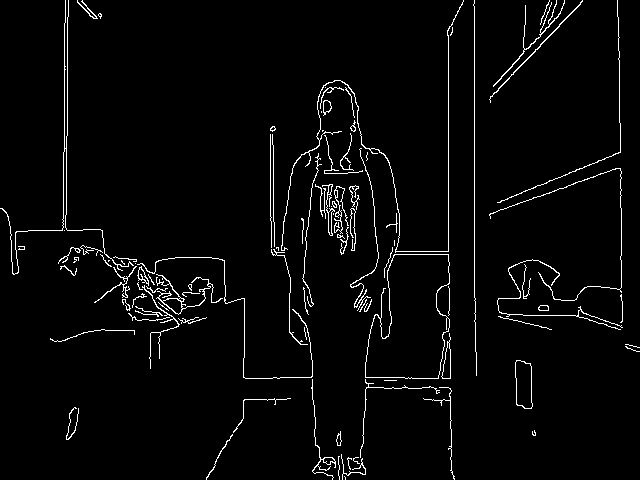
\includegraphics[width=8cm]{canny.jpg}
  \caption{图像边缘提取图\label{fig:6}}
\end{figure}

最后还要对每个手势阶段的所有的运动图像边缘进行一个历史叠加,就得到了每个状态的运动信息,如图\ref{fig:7},这里面包含了远多于CNN网络提取到的动作特征,因此认为是高级动作特征,然后我们对提取到的特征进行k-means聚类就得到包含k个聚类中心的单词表。

\begin{figure}[ht]
  \centering
  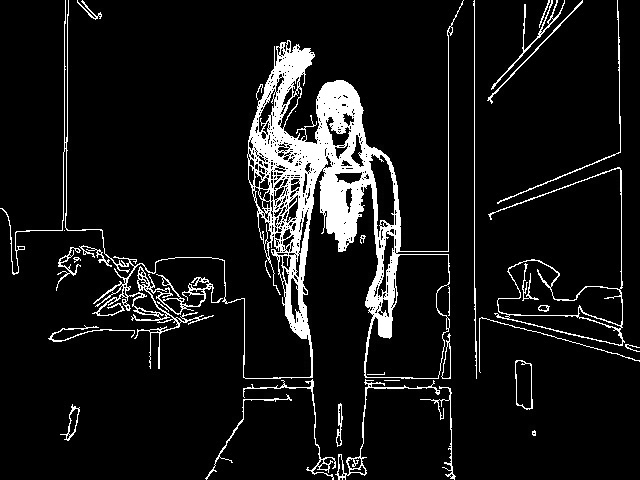
\includegraphics[width=8cm]{combineresult.jpg}
  \caption{\label{fig:7}历史边缘叠加图}
\end{figure}

\subsubsection{动态调整输入帧步长}
原方法的网络输入为连续帧,改进方法将输入帧步长分别设置为1、2和4,根据训练手势序列的长度做动态调整。

\section{实验设置}
\subsection{实验数据集}
本实验使用的数据集为2014年ChalearnLAP手势识别挑战赛中公开发布的数据集。该数据集包含940条视频序列,每条视频序列包含10至20个手势,并由一个人独立完成,完整数据集包含来自20个手势类别的近14000个手势片段。其中每个手势的平均长度为39个视频帧,持续最短的手势持续时长为16帧,持续最长的手势为104帧。数据集包含了三种模态的数据:骨骼数据(全身20个关节位置坐标、旋转角度以及像素坐标),RGB图像以及深度图像(还包含二值化灰度图),标签中包含了手势类别以及该手势的起始帧和终止帧。将数据集的内容可视化如下图所示:

\begin{figure}[ht]
  \centering
  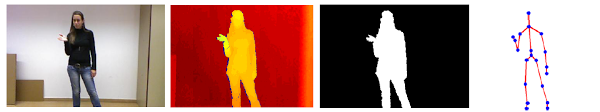
\includegraphics[width=8cm]{dataVisual.png}
  \caption{\label{fig:8}可视化数据集}
\end{figure}

这一项挑战的难点在于识别结果要做到“用户独立”,不同的人做相同的手势动作也会略有不同。除此之外,有些手势的手臂动作很相似,只在手部动作上略有不同,这也造成了一定的识别难度。

\subsection{实验设置}
实验采用数据和可视化图像相结合的方式多方位地评估模型表现,对比了方法改进前后性能的提升,并附上了本文方法与其他众多先进方法的性能对比。


\subsection{评价标准}
我们采用Jaccard指数来评估识别效果,对于每一段视频序列,Jaccard指数的定义如下:

\begin{equation}
J_{s,n} = \frac{A_{s,n} \bigcap B_{s,n}}{A_{s,n} \bigcup B_{s,n}}
\end{equation}

其中,$A_{s,n}$代表正确标注,$B_{s,n}$表示预测序列。最终的评估结果用所有视频序列Jaccard指数的平均值来表示:
\begin{equation}
J_{mean} = \frac{1}{|G_i|}\sum_{G_i}J_{s,n}
\end{equation}


除此之外,我们还采用了PASCAL标准,
对一个手势块G,以及它的识别结果R,用$\frac{G\cap R}{G\cup R}$来评估预测表现。



\section{实验结果分析}
\subsection{原方法实验结果}
本文方法的综合评估情况如表\ref{tab:1}所示,其中列出了两个单独模块对验证集和测试集的预测情况,以及两种融合模型的预测表现。可以看到,骨骼网络对手势的预测准确性要高于RGB-D网络,融合网络的预测准确率以及泛化能力相较于两个独立的模块又进一步提升。另一个值得注意的是,骨骼数据的误识别情况明显高于漏识别的情况,而RGBD的情况刚好相反,漏识别的比例远高于误识别的比例。这个问题很好定性的来解释,骨骼数据对动态特性的分析能力较强,而图像数据则对外观信息更为敏感,手势集中的有些动作比较相近的手势,他们仅在手的姿态上略有不同,这就很容易导致骨骼网络发生混淆,而RGBD网络则对这种情况的处理能力优于前者。
\begin{table}[htbp]
 \caption{\label{tab:1}本文各模型识别性能比较}
 \centering
 \begin{tabular}{lccl}
  \toprule
    & \% & 验证集 & 测试集\\
  \midrule
 Skeleton-DBDN & 识别 & 86.3 & 83.6\\
               & 误识别 & 11.4 & 12.3\\
               & 漏识别 & 2.3 & 4.1\\
 RGB-D-3DCNN & 识别 & 78.7 & 75.8\\
               & 误识别 & 5.2 & 4.5\\
               & 漏识别 & 16.1 & 19.7\\
 Multimodal Late Fusion & 识别 & 87.9 & 86.4\\
               & 误识别 & 9.1 & 8.7\\
               & 漏识别 & 3.0 & 4.9\\
 Multimodal Inter. Fusion & 识别 & 86.5 & 85.5\\
               & 误识别 & 7.3 & 6.8\\
               & 漏识别 & 6.2 & 7.7\\
  \bottomrule
 \end{tabular}
\end{table}

用混淆矩阵的方式能够更直观地展示不同模型的预测性能,如图\ref{fig:9}。
\begin{figure} \centering
\subfigure[骨骼模型] { \label{fig:9a}
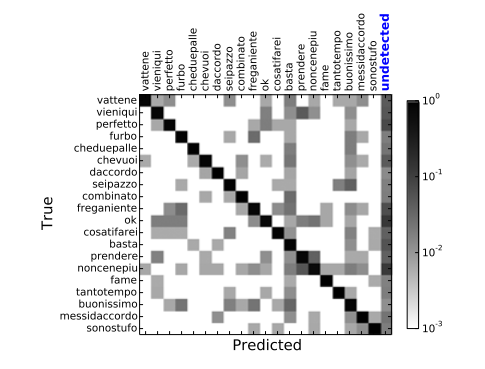
\includegraphics[width=6cm]{cm_sk.png}
}
\subfigure[RGB-D模型] { \label{fig:9b}
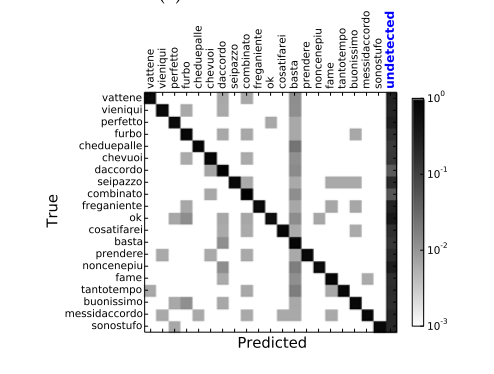
\includegraphics[width=6cm]{cm_rgb.png}
}
\subfigure[融合模型] { \label{fig:9c}
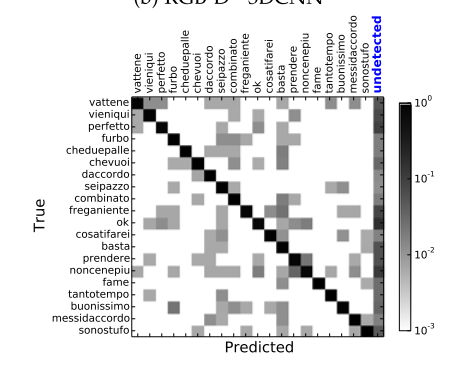
\includegraphics[width=6cm]{cm_fu.png}
}
\caption{\label{fig:9}本文各模型的混淆矩阵}
\end{figure}

\subsection{改进方法实验结果}
本文的改进主要是在CNN网络这一块,通过提高RGBD模块的预测准确性,进而提高了整体模型的准确性,因此实验主要关注CNN网络的效果提升。CNN网络存在较多漏识别的最根本原因是提取的特征不够强大,不足以用来识别跨域了多帧的高级行为信息。在我们引入高级行为特征向量来对模型进行规则化以后,得到了对验证集的混淆矩阵如图\ref{fig:10}所示,对比图\ref{fig:9}中改进前的混淆矩阵,能够观察到漏识别一栏的颜色深度有所下降。
\begin{figure}[ht]
  \centering
  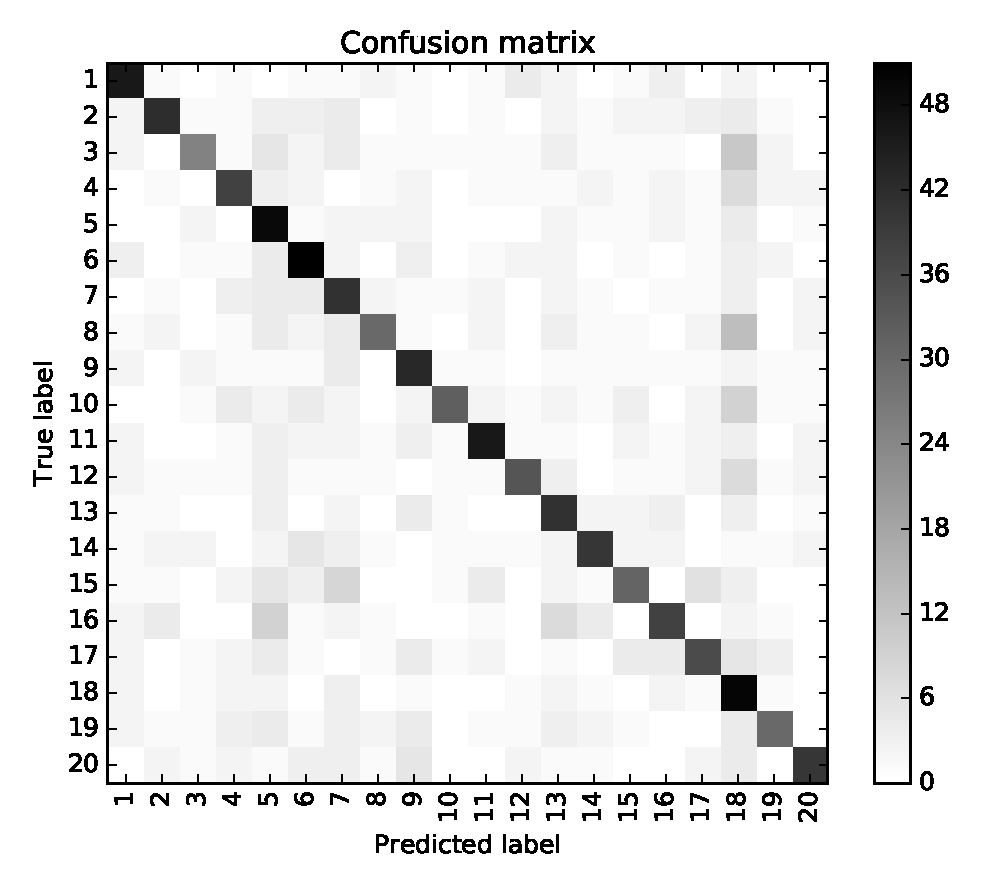
\includegraphics[width=8cm]{cmnorm.eps}
  \caption{\label{fig:10}改进CNN的混淆矩阵}
\end{figure}

本文随机抽取了几段视频,利用改进前后的预测结果对其中的手势序列进行标注,对比结果如图\ref{fig:11},可以看到有一部分在改进前没有识别到的手势在改进后被成功识别了出来。
\begin{figure} \centering
\subfigure[] { \label{fig:9a}
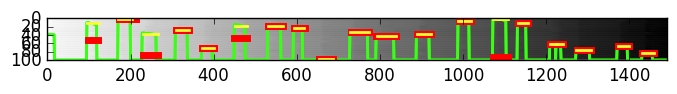
\includegraphics[width=6cm]{raw0463.png}
}
\subfigure[] { \label{fig:9b}
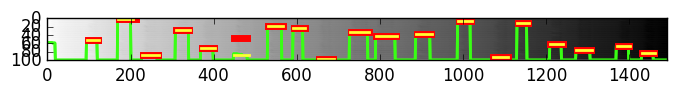
\includegraphics[width=6cm]{enhance0463.png}
}
\subfigure[] { \label{fig:9c}
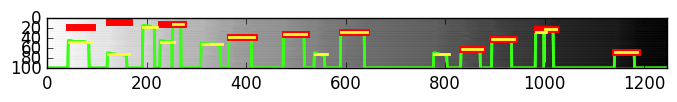
\includegraphics[width=6cm]{raw0465.png}
}
\subfigure[] { \label{fig:9d}
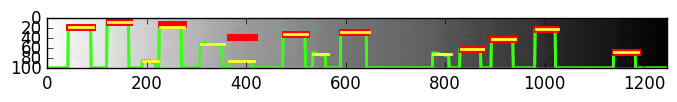
\includegraphics[width=6cm]{enhance0465.png}
}
\caption{\label{fig:11}预测标注序列}
\end{figure}

\section{结论}
3D-CNN的方法虽然较传统的2D的方法增加了时间轴,考虑到了对动态特征的提取,但是由于输入窗口尺寸有限在分析高级运动特征的时候还是具有一定的局限性。本文通过引入动态目标的边缘信息来获取高级行为信息,用已知的高级运动特征来引导CNN网络的规则化输出,提升算法表现。相较于原方法的简单叠加,对双通道的运动特征予以保留也在一定程度上使得网络性能更好。本文还兼顾到了控制计算量的问题,动态调整输入帧的步长,提升学习效率。总体来说,改进方法较原方法具有性能提升。

\section*{致谢}
我要在此特别感谢指导老师尤明宇老师,在本论文撰写过程中给予我悉心的指导,使我能够克服重重困难,将实验与论文完成。


\bibliography{bib}

\end{document}
